\definecolor{rsgreen}{HTML}{2F855A}
\definecolor{rsamber}{HTML}{D97706}
\definecolor{rsred}{HTML}{C2413A}
\definecolor{rsink}{HTML}{334155}
\definecolor{rsmuted}{HTML}{64748B}
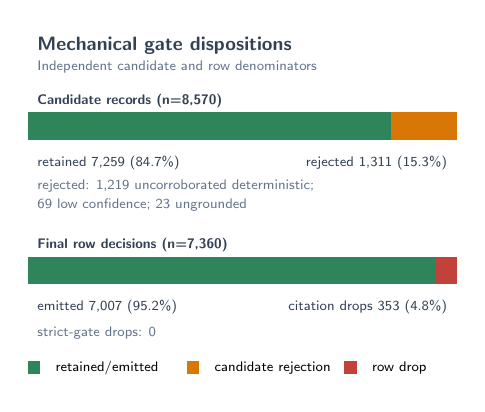
\begin{tikzpicture}[x=1cm,y=1cm,every node/.style={font=\sffamily}]
\node[anchor=west,font=\sffamily\scriptsize\bfseries,text=rsink] at (0,4.25) {Mechanical gate dispositions};
\node[anchor=west,font=\sffamily\tiny,text=rsmuted] at (0,3.98) {Independent candidate and row denominators};

\node[anchor=west,font=\sffamily\tiny\bfseries,text=rsink] at (0,3.55) {Candidate records (n=8,570)};
\fill[rsgreen] (0,3.05) rectangle (4.616,3.40);
\fill[rsamber] (4.616,3.05) rectangle (5.450,3.40);
\node[anchor=west,font=\sffamily\tiny,text=rsink] at (0,2.76) {retained 7,259 (84.7\%)};
\node[anchor=east,font=\sffamily\tiny,text=rsink] at (5.450,2.76) {rejected 1,311 (15.3\%)};
\node[anchor=west,font=\sffamily\tiny,text=rsmuted] at (0,2.47) {rejected: 1,219 uncorroborated deterministic;};
\node[anchor=west,font=\sffamily\tiny,text=rsmuted] at (0,2.22) {69 low confidence; 23 ungrounded};

\node[anchor=west,font=\sffamily\tiny\bfseries,text=rsink] at (0,1.72) {Final row decisions (n=7,360)};
\fill[rsgreen] (0,1.22) rectangle (5.189,1.57);
\fill[rsred] (5.189,1.22) rectangle (5.450,1.57);
\node[anchor=west,font=\sffamily\tiny,text=rsink] at (0,0.93) {emitted 7,007 (95.2\%)};
\node[anchor=east,font=\sffamily\tiny,text=rsink] at (5.450,0.93) {citation drops 353 (4.8\%)};
\node[anchor=west,font=\sffamily\tiny,text=rsmuted] at (0,0.60) {strict-gate drops: 0};

\fill[rsgreen] (0,0.08) rectangle (0.16,0.24);
\node[anchor=west,font=\sffamily\tiny] at (0.23,0.16) {retained/emitted};
\fill[rsamber] (2.02,0.08) rectangle (2.18,0.24);
\node[anchor=west,font=\sffamily\tiny] at (2.25,0.16) {candidate rejection};
\fill[rsred] (4.02,0.08) rectangle (4.18,0.24);
\node[anchor=west,font=\sffamily\tiny] at (4.25,0.16) {row drop};
\end{tikzpicture}
